\chapter{Аналитический обзор}
\label{mainpart} 
\section{Обзор объекта исследования}

Теоретические исследования в области построения математических моде\-лей процесса выполнения заданий играют огромную роль в современных системах компьютерного обучения. Одним из
вопросов, которые исследуются в данной области является взаимосвязь между временем ответа студента и правильностью ответа.

Наиболее ранние работы в данной области принадлежат Вудбори (Woodbury) (1951, 1963), который использовал стохастические модели для коли\-чества правильных ответов, предоставленных студентом в течении теста. Поз\-днее эти идеи были развиты в работах  Лорда и Новика (Lord, Novick) (1968).

В этот период так же возникла идея о том, что оценка студента не должна складываться только из количества правильных ответов, предоставленных в течение теста - необходимо учитывать и время, которое студент затрачивает на решение задачи. Эти вопросы поднял в своих работах Галексен (Gulliksen) (1950). Он предложил использовать два вида тестов - тесты на скорость (speed tests) и тесты на сложность задач (power tests). При прохождении теста на скорость студенту предлагалось за ограни\-ченное время решить макси\-мально возможное количество задач самого низ\-кого уровня - таким образом Галексен пытался оценить скорость, с которой студеты принимают решения, при этом на скорость ответов не должна влиять сложность задачи. Тесты второго вида состояли из задач разного уровня сложности, время на решение которых было неограничено - по результатам этого теста можно было оценить, задачи какого уровня сложности может решить студент, т.е. оценить именно уровень знаний, без привязки к скорости, с которой обучающийся решает задачи.

 Подход Галексена обладает двумя основными недостатками: во-первых даже в тестах на скорость может случиться так, что на какую-то из задач студент даст неверный ответ (это маловероятно для студентов с высоким уровнем знаний, но вполне может произойти с менее способными студентами). Как в данном случае оценить скорость студента с помощью времени ответа, как учесть время, за которое студент дал неверный ответ и нужно его учиты\-вать вообще? Во-вторых, здравый смысл подсказывает, что время нужно учитывать так же и в тестах на сложность задач - ведь если два студента решают все предложенные задачи, но один из них при этом затрачивает меньшее количество времени - очевидно, что "быстрый" студент заслуживает более высокую оценку.

 Одним из первых исследователей, который пытался решить даные за\-дачи, был Терстоун (Thurstone) (1937). Он обратил своё внимание на воп\-рос взаимосвязи между скоростью, с которой студент решает задачи и теста и уровнем знаний студента. Терстоун представил графическую модель такой взаимосвязи, которую назвал "кривой ответа" (response surface). Для каждого конкретного студента и одной задачи теста кривая ответа представляет собой график зависимости вероятности правиль\-ного ответа от сложности задачи и времени, которое было затрачено на ответ. Пример кривой ответа показан на рисунке ниже

\begin{figure}[ht!] 
\centering 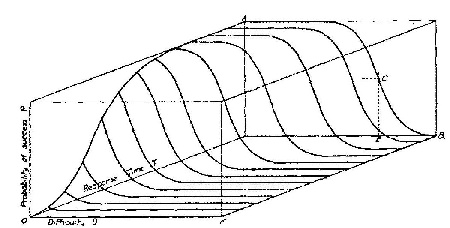
\includegraphics[bb=0 0 450 228]{6.jpeg} 
\caption{Кривая ответа} 
\end{figure}

График отражает зависимость между вероятностью правильного ответа и затраченным временем только для одного студента, т.е. не отражает распре\-деление вероятности для группы студентов. Основной принцип, который Тер\-стоун использовал при построении этой диаграммы: вероятность того, что студент даст правильный ответ на задачу растёт с увеличением времени, которое студент затратит на задачу. При этом вероятность правиль\-ного ответа уменьшается с увеличением сложности задачи. Терстоун ввёл понятия ско\-рости студента и способностей студента. Скорость студентов Терстоун опре\-делил как число задач, которые студент решает в единицу времени; способ\-ностю студента исследо\-ватель назвал сложность задач, на которые студент отвечает с вероятностью $P=0.5$ при условии, что время ответа студента не ограничи\-вается.

Несмотря на достоинства, в модели Терстоуна есть так же и некоторые неочевидные недостатки. Во-первых, для ответов студента используется сто\-хастическая модель, в то время как время ответа считается детерминирован\-ным. Очевидно, что и ответы студента и время, которое студент затрачивает на ответ являются следствиями одних и тех же когнитивных процессов - поэтому логично использовать вероятностную модель так же и для времени ответа студента. Таким образом, кривая ответа должна преставлять собой закон совместного распределения времени ответа и корректных ответов сту\-дента. Во-вторых, модель Терстоуна принимает в качестве параметров веро\-ятностной модели ответа парамет\-ры задачи (сложность) и параметры сту\-дента (способность), при этом игнорируется время, в течении которого студент отвечал на задание. Во-третьих, кривая ответа предпола\-гает зависимость ве\-роятности правильного ответа от времени ответа, в то время как логично предположить, что между этими величинами существует условная незави\-симость, т.е. ответ на задачу и время ответа на любую задачу теста не должны зависеть от ответов на другие задачи. 

Таким образом, при изучении вопросов обучения студентов исторически возникли такие задачи, как
\begin{itemize}
\item оценить способность каждого студента
\item оценить скорость, с который конкретный студент может решить пред\-ложенную задачу теста
\item оценить время, которое может потребоваться студенту для полного про\-хождения теста
\item сформировать список задач, который будет оптимальным для конкрет\-ного студента, исходя из его способностей
\end{itemize}
и другие.

Дипломная работа посвящена построению математической модели времени ответа студента и одному из практических применений этой модели: выявлении отклонений в поведении студента на основании поступающей в систему дистан\-ционного обучения информации о времени ответа студента на задачи теста.

\section{Предмет дипломной работы}

Предметом дипломной работы является время, которое студент затрачи\-вает при ответе на вопросы теста. Очевидно, что время ответа играет важную роль при оценке уровня способностей студента и формирования индивидуаль\-ных заданий в системе дистанционного обучения: например, два студента с одина\-ковым уровнем подготовки  могут отвечать на вопросы теста с разной скоростью - это значит, что при одинаковых ограничениях на общее время на теста более "медленный" студент не успеет ответить на все задачи.

В связи с этим возникает необходимость в моделировании времени ответа студента. Информация о времени, которое ожидается при ответе студента на данную задачу может использоваться системой дистанционного обучения для различных целей: например, для адап\-тации индивидуального задания согласно возможностям конкретного студента. Матема\-тическая модель времени ответа студента на задачи позволяет ответить на следующие вопросы:
\begin{itemize}
\item уложится студент во время, отведённое на тест для конкретного набора задач
\item не пытается ли студент во время теста угадать ответ вместо того, чтобы решать задачу
\item не пользуется ли студент готовыми решениями, полученными ранее
\item понять стратегию, которую студент использует  во время ответов на задачи
\end{itemize}

Для решения этих задач существует множество теоретических моделей, которые\\ рассматриваются далее в Главе \ref{ch2}.
